\documentclass{article}
\usepackage[utf8]{inputenc}
\usepackage{mathtools}

\newcommand{\avg}[1]{\langle#1\rangle}
\title{Experimental demonstration of the relationship between CHSH and Instrumental inequalities}
\begin{document}
\maketitle

\section*{Instrumental and CHSH}
\begin{figure}[h]
    \centering
    \parbox{.4\textwidth}{
        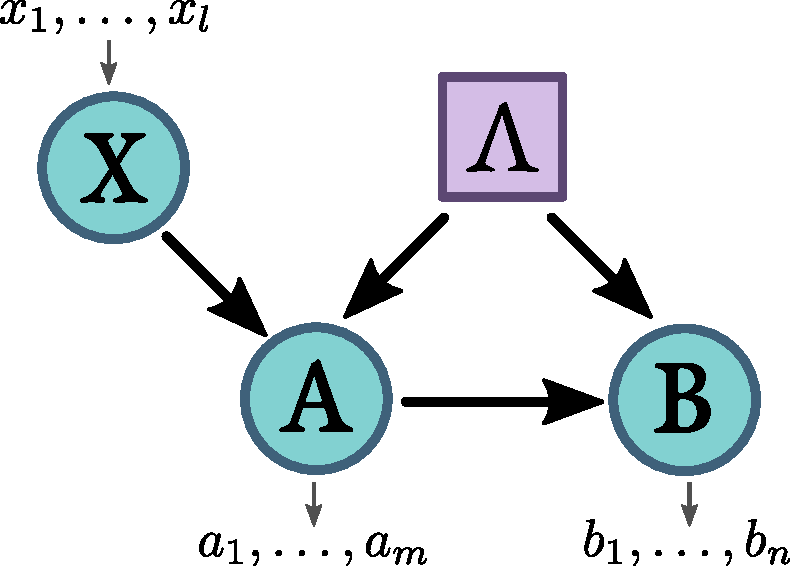
\includegraphics[width=.4\textwidth]{images/instdag.pdf}
        \caption{The DAG representing a general Instrumental scenario.}
        \label{fig:instdag}
    }
    \qquad
    \parbox{.4\textwidth}{
        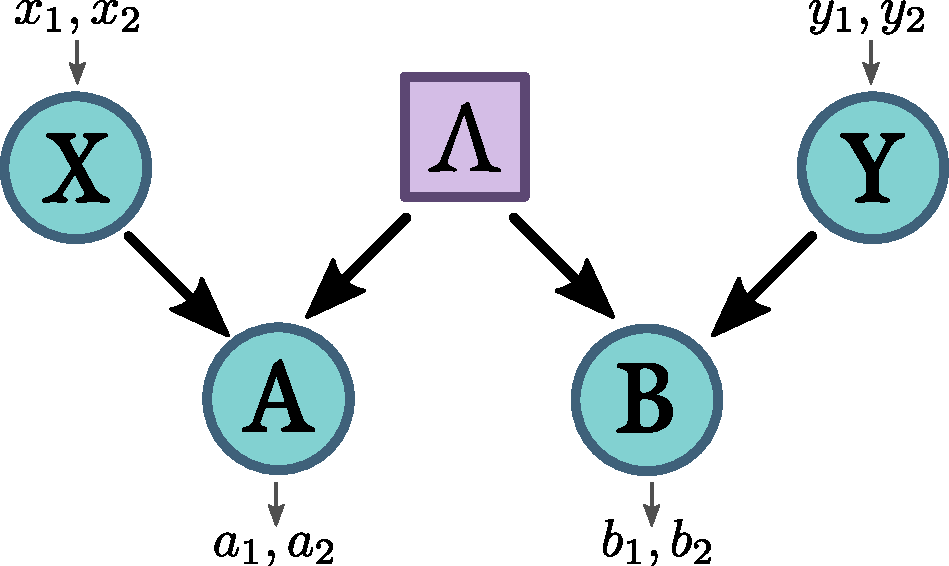
\includegraphics[width=.4\textwidth]{images/chshdag.pdf}
        \caption{The DAG representing a general Instrumental scenario.}
        \label{fig:chshdag}
    }
\end{figure}

The so-called ``Instrumental'' causal structure is a widely studied
structure both for its simplicity and commonness.
It can be described by four random variables $\Lambda, X, A, B$ where $X$ and
$\Lambda$ are independent of the others and $B$ depends on $X$ only through $A$,
as graphically depicted in fig.~\ref{fig:instdag}.

The consequences of these causal relations on the distributions of the four
variables have been throughly studied in previous works \cite{pearl1995,
bonet2001}.
Suppose that $X, A, B$ can take $l,m,n$ different values and 
call $P(a_i b_j | x_k)$ the probability that $A$ and $B$ take values $a_i$
and $b_j$ respectively, given that $X$ takes value $x_k$.
Bonet \cite{bonet2001} pointed out that the polytope of allowed
correlation is characterized not only by the \emph{Pearl's inequalities}:
\begin{equation}
    \sum_{j=0}^{n} P(a_i b_j|x_{k(i,j)}) \le 1
    \label{eq:pearl_ineq}
\end{equation}
for all $i \in {1,\ldots, m}$ and for all the possible functions $k(i,j)$.
For example for $(l,m,n) = (3,2,2)$ the inequality:
\begin{equation}
    P(a_1 b_1 | x_1) + P(a_2 b_2 | x_1) + 
    P(a_1 b_1 | x_2) + P(a_2 b_1 | x_2) + 
    P(a_1 b_2 | x_3) \le 2
    \label{eq:bonet_ineq}
\end{equation}
must also be satisfied, along with other similar inequalities.

These inequalities are closely related to the one presented in \cite{chaves2018}:
\begin{equation}
    -\avg{B}_{x_1} + 2 \avg{B}_{x_2} + \avg{A}_{x_1} - \avg{AB}_{x_1} +
    2\avg{AB}_{x_3} \le 3  
    \label{eq:rafael_ineq}
\end{equation}
which, as was recently experimentally violated in the same work, and admits a
quantum violation of $3.79 \pm 0.013$.
As one can expect, with the same data we can also violate inequality
\eqref{eq:bonet_ineq} with a value of $2.159$.

A similar analisys can be done in the CHSH scenario, depicted in
fig.~\ref{fig:chshdag},
where the variables all have two possible outcomes.
Here instead we have the notorious inequality:
\begin{equation}
    \avg{A_1B_1} + \avg{A_1B_2} + \avg{A_2B_1} - \avg{A_2B_2} \le 2
    \label{eq:chsh_ineq}
\end{equation}

As was pointed out in \cite{himbeeck2018} these two scenarios (CHSH and the Instrumental)
are somewhat related, and indeed, in a sense, the two quantum violations can be
seen as a consequence of one another.
To see this we must can think of the Instrumental scenario as a restricted CHSH,
where we postselect in the case of $Y = A$, and we augment the variable $X$ with
an additional value $x_3$ as described in \cite{himbeeck2018}.
From this analisis the maximum quantum violation would be $(3 + \sqrt{2})/2$.

\begin{figure}[h]
    \centering
    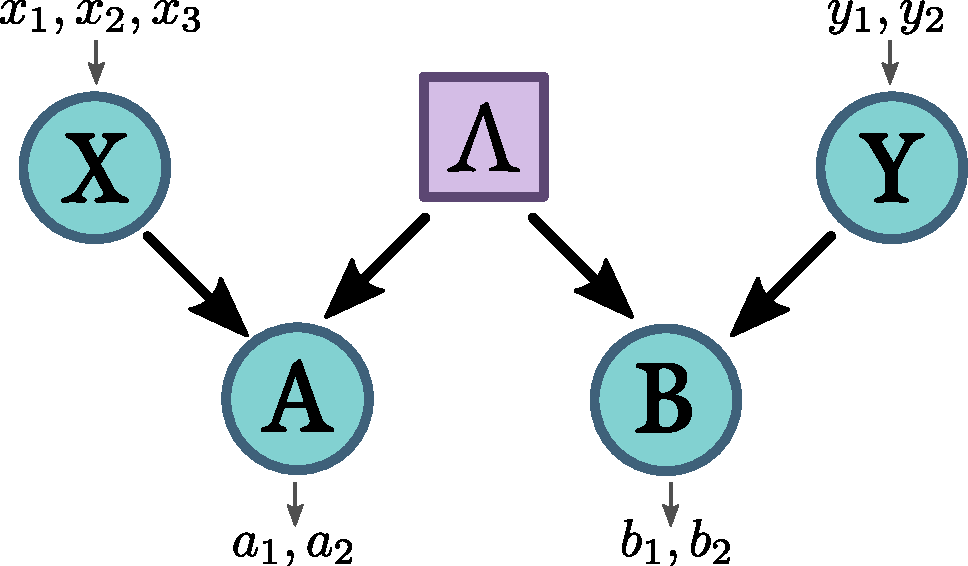
\includegraphics[width=.5\textwidth]{images/genchshdag.pdf}
    \caption{A generalization of the CHSH DAG.}
    \label{fig:genchshdag}
\end{figure}
This can be verified experimentally provided we have an apparatus capable of
reproducing the causal structure depicted in fig.~\ref{fig:genchshdag} i.e. a CHSH scenario
where $X$ can take 3 possible values, as the apparatus presented in
\cite{chaves2018}.
Taking advantage of this we can violate all three inequalities
\eqref{eq:bonet_ineq}, \eqref{eq:rafael_ineq} and \eqref{eq:chsh_ineq} with the same set of
data:
\begin{enumerate}
    \item To violate the Instrumental inequalities we postselect in the case
        $Y = A$, obtaining values $3.79 \pm 0.013$ and $2.159$ for \eqref{eq:rafael_ineq} and
        \eqref{eq:bonet_ineq} respectively.
    \item To violate the CHSH inequality we just ignore the case $X = x_3$,
        obtaining the value $2.619 \pm 0.005$.
\end{enumerate}

\section*{Instrumental and contextuality}
\begin{figure}[h]
    \centering
    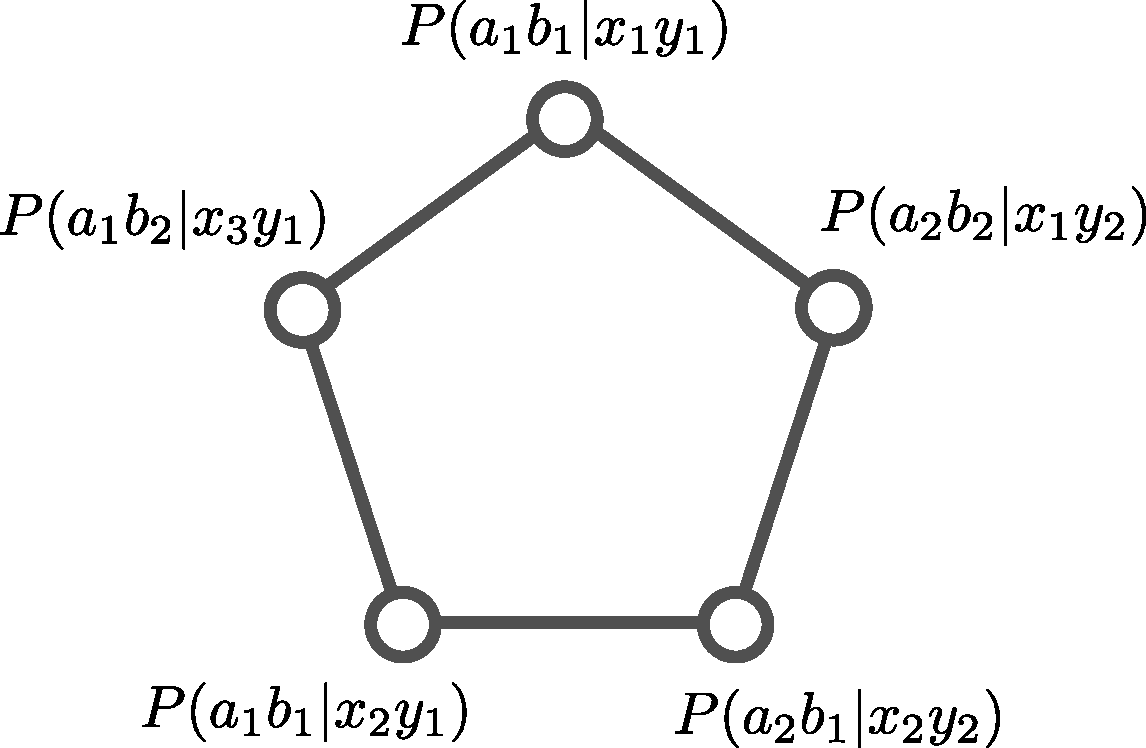
\includegraphics[width=.6\textwidth]{images/bonetexc.pdf}
    \caption{The exclusivity graph of the bonet inequality.}
    \label{fig:bonetexc}
\end{figure}
Interestingly the inequality \eqref{eq:bonet_ineq} can also be obtained using
the methods presented in \cite{cabello2014}.  Indeed, following
\cite{cabello2014}, the exclusivity structure of the events in
\eqref{eq:bonet_ineq}, form a $C_5$ cyclic graph, i.e. the pentagon depicted in
fig.~\ref{fig:bonetexc}, so that the classical limit would be $2$.
In this framework \eqref{eq:bonet_ineq} is analogous to the KCBS contextual
inequality.
Nonetheless the quantum limit for the KCBS is $\sqrt{2}$ \cite{cabello2014}, different
from the limit expected for the Bonet inequality found in \cite{himbeeck2018}.
This is probably due to the fact that the KCBS limit is attained with a
particular configuration of projectors in 3D space, while in the
Instrumental scenario the only possible projectors are necessarly tensor product of
projectors in two 2D space.
It would be interesting to see if the same limit $\sqrt{5}$ can be obtained in the
Instrumental scenario, maybe in a generalized context where $X$ is not
tricothomic, and if the other inequalities for the Instrumental scenario
presented in \cite{bonet2001} can be obtained as contextual inequalities.

\begin{thebibliography}{}
    \bibitem{pearl1995} J.Pearl, {\em On the testability of causal models with
        latent and instrumental variables}, 
        Proceedings of the Eleventh conference on Uncertainty in artificial
        intelligence. Morgan Kaufmann Publishers Inc. (1995).
    \bibitem{bonet2001} B.Bonet, {\em Instrumentality tests revisited},
        Proceedings of the Seventeenth conference on Uncertainty in artificial
        intelligence. Morgan Kaufmann Publishers Inc. (2001).
    \bibitem{chaves2018} R.Chaves, G.Carvacho, I.Agresti, V.Di Giulio, L.Aolita,
        S.Giacomini, F.Sciarrino, 
        {\em Quantum violation of an instrumental test}, 
        Nature Physics 14.3 291 (2018).
     \bibitem{himbeeck2018} T.Van Himbeeck, J.B. Brask, S.Pironio, R.Ramanathan, A.B.Sainz, E. Wolfe, 
        {\em Quantum violations in the Instrumental scenario and their relations to the Bell scenario},
        arXiv preprint arXiv:1804.04119 (2018).
         (2014). . 
     \bibitem{cabello2014} A.Cabello, S.Severini, A.Winter,
         {\em Graph-theoretic approach to quantum correlations}, 
         Physical review letters, 112(4), 040401 (2014).
%\bibitem{} , {\em },  ().
\end{thebibliography}

\end{document}
